\documentclass[a4paper]{article}

\usepackage[english]{babel}
\usepackage[utf8x]{inputenc}
\usepackage{amsmath}
\usepackage{amsfonts}
\usepackage{graphicx}
\usepackage[colorinlistoftodos]{todonotes}

\title{CS 5785 -- Applied Machine Learning -- Lec.\ 22}
\author{Prof.\ Nathan Kallus, Cornell Tech\\Scribe: TBD}
\date{Fall, 2017 (Under construction)}

\begin{document}
\maketitle
\todo[inline]{rough draft -- still needs editing}

\section{Review of SVMs from Last Time}

Recall we're looking at a simplified case with two separable classes.  There are an infinite number of lines separating the two classes; the optimal separating hyperplane (the one that probably generalizes the best to testing data) is the one with the maximum margin.

You can formulate the maximum margin with a convex optimization problem. There are two parts: a quadratic term and a constraint term.  It starts off with a quadratic criterion with linear inequality constraints and write the Lagrange (primal) function, to be minimized with regard to $\beta$ and $\beta_0$ as:
$$
L_p = \frac{1}{2}||\beta||^2-\sum_{i=1}^N\alpha_i[y_i(x_i^\top\beta+\beta_0)-1]
$$

This basically takes the constraint and turns it into weighted penalties.

\section{Deriving the SVM}

To solve this problem, set the derivative with respect to $\beta_1$, $\beta_0$ equal to zero.

\begin{align}
\beta &= \sum_{i=1}^{N} \alpha_i y_i x_i\\
0 &= \sum_{i=1}^{N} \alpha_i y_i
\end{align}

Recall that $\|\beta\|^2 = \beta^\top \beta$. So $\frac{1}{2} \frac{d}{d\beta} \|\beta\|^2 = \beta$ thinking about doing a derivative with vectors.  This is telling us that the coefficients are a linear combination of all observations weighted by $\alpha$ and the label.  If you plug $\beta$ back into the expression for $L_p$ you get the ``Wolfe dual'':

\begin{align}
L_D = \sum_{i=1}^{N} \alpha_i - \frac{1}{2} \sum_{i=1}^{N} \sum_{k=1}^{N} \alpha_i x_k y_i y_k x_i^\top x_k \;
\text{ subject to } \alpha_i \geq 0
\end{align}

The $x_i^\top x_k$ in the above equation is an inner product that can be swapped in for a kernel instead, which is a generalization of a dot product.

We get the solution by maximizing $L_D$ in the \emph{positive orthant}, i.e. $\alpha_i \geq 0$, a simple convex optimization problem for which standard solvers can be used.

The solution must also satisfy the Karush-Kuhn-Tucker (KKT) conditions which consist of Equations (1), (2), (3), and below (4).

\begin{align}
\alpha_i [y_i (x_i^\top \beta + \beta_0) -1] = 0 \; \forall i
\end{align}

This tells us that:
\begin{enumerate}
\item If $\alpha_i > 0$ then $y_i (x_i^\top \beta + \beta_0) =1$, i.e. $X_i$ is on the boundary of the slab, as seen in Fig. ~\ref{fig:svm1}. 
\item If $y_i (x_i^\top \beta + \beta_0) > 1$, $x_i$ is not on the boundary of the slab, and $\alpha_i=0$.
\end{enumerate}

\begin{figure}
\centering
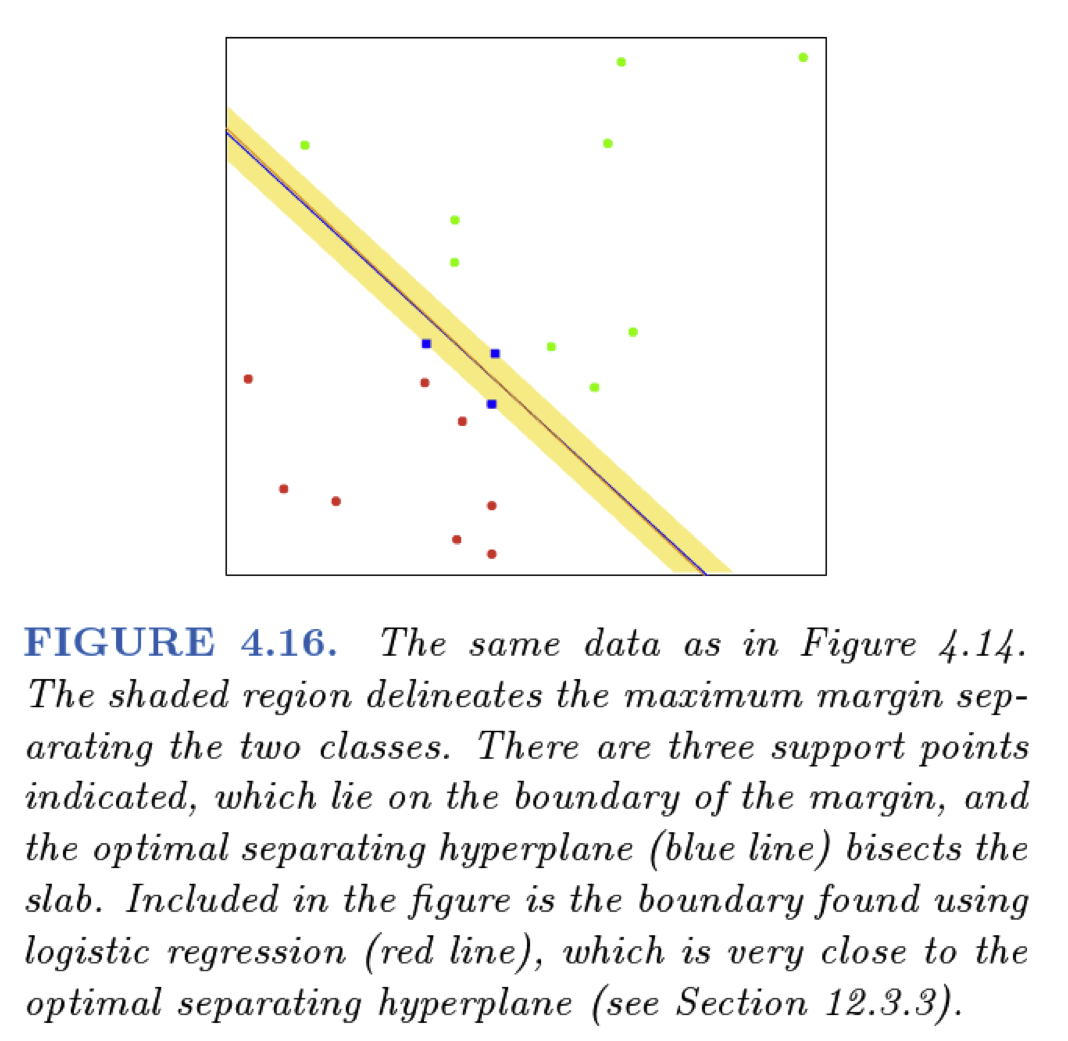
\includegraphics[width=1.0\textwidth]{fig4_16.png}
\caption{\label{fig:svm1}Figure 4.16}
\end{figure}

From Equation (1) we see that $\beta$ is defined as a linear combination of the support points $\alpha_i$.

We get $\beta_0$ by solving for Equation (4) for any of the support points.  Finally, the optimal separating hyperplane is given by:

\begin{align*}
\hat{f}(x) &= x^\top \beta + \beta_0 \\
\hat{G}(x) &= sign \; \hat{f}(x)
\end{align*}

Every point in the data set has the potential to have a non-zero $\alpha$ but the data points that contribute to the separating hyperplane are the ones on the margin, on the periphery of the slab.  This is extremely efficient since most of the points are zero and don't contribute to the decision.  You get $\beta$ and the offset $\beta_0$ and then threshold it to get the final decision.

Let's compare this with LDA and logistic regression, assuming a 2-class problem that's separable.  For LDA, we assume the classes are distributed as bivariate Gaussians that have the same means but different covariances.  But it's probably not the case that your data is like this  For logistic, you also get a decision line or hyperplane using not the points themselves but with log-odds as a linear combination.  Logistic is pretty similar qualitiatively to SVM because we get driven to two extreme values.  In Newton-Raphson, the coefficents are most important close to the boundary.  All points become support vectors or not, so $\alpha=0$ or $\alpha \neq 0$.

\section{Non-separable Hyperplanes}

What do you do when the data is not separable (not some slab away from a hyperplane)?

\begin{figure}
\centering
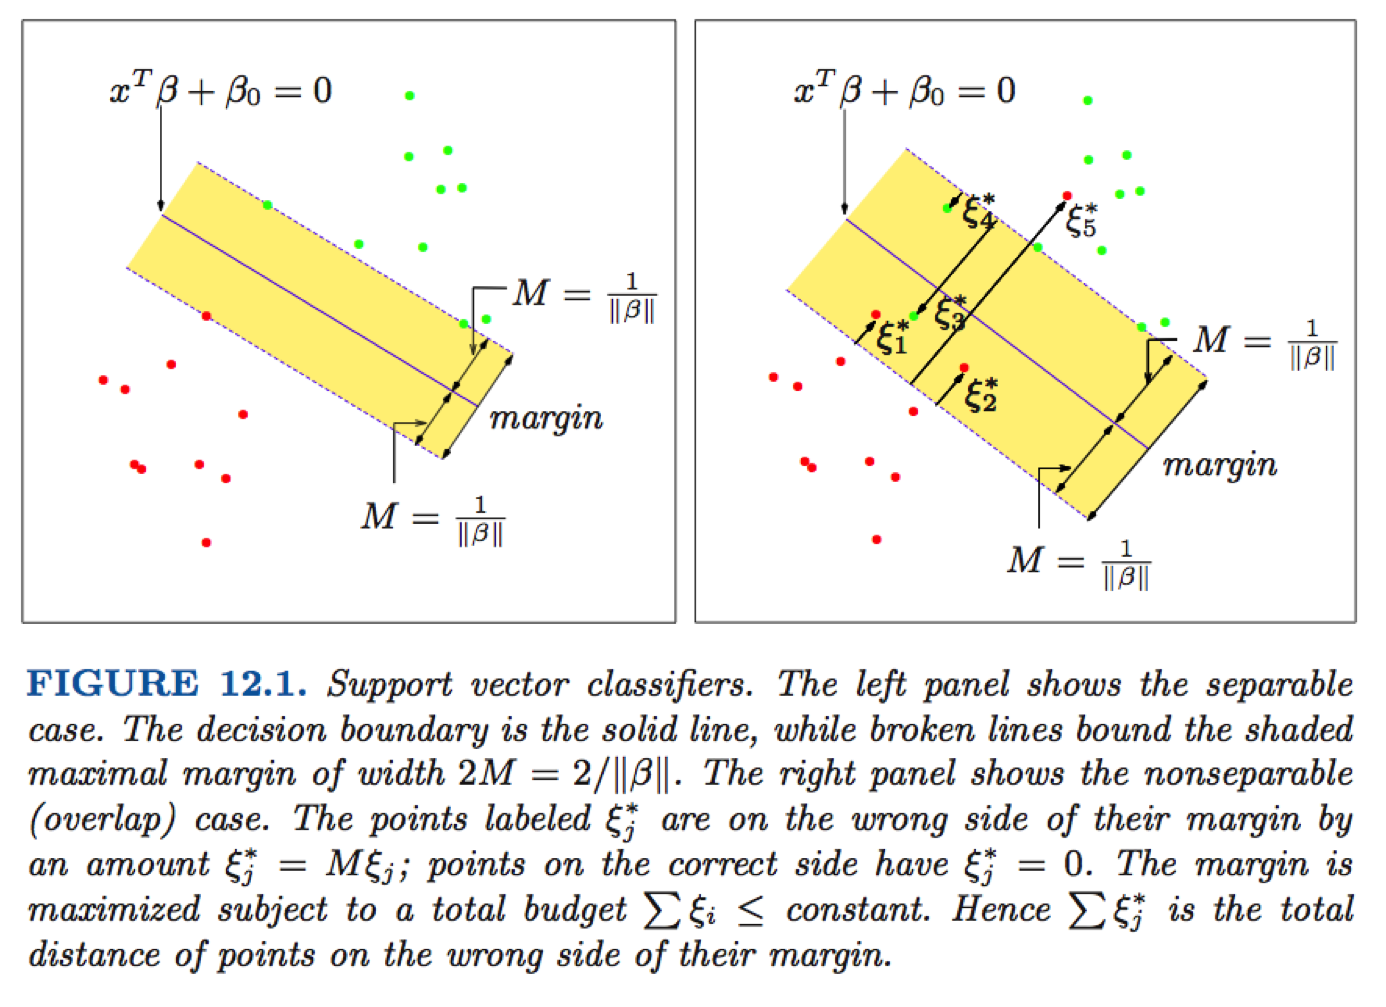
\includegraphics[width=1.0\textwidth]{fig12_1.png}
\caption{\label{fig:svm2}Figure 12.1}
\end{figure}

We won't do derivations for this non-separable case but we will talk about this, as seen in ~\ref{fig:svm2}.  When you look at the non-separable case, you think that have a margin that is a perfectly separating margin and have some points on the wrong side of the boundary.  You attach to every single data point a slack variable, $\xi_i$.  The slack variable has the ability to move into the correct side like a rubber band, if you're willing to pay the price.

However, we may overfit if the slack variables are left unconstrained.  The amount of stretch is specified by the variable $c$, a regularization constant, which we last saw with decision trees.  We want a compromise allowing some data points to have slack.  The regularization is like having a budget for the slack variables.  If $c=0$ then you're not constraining anything.  If $c$ is really big, you're being very inflexible assuming that nothing is allowed to violate the constaint, on the left, which is very inflexible.  You can use cross-validation to find c.  Fig. ~\ref{fig:svm3} shows an example.

\begin{figure}
\centering
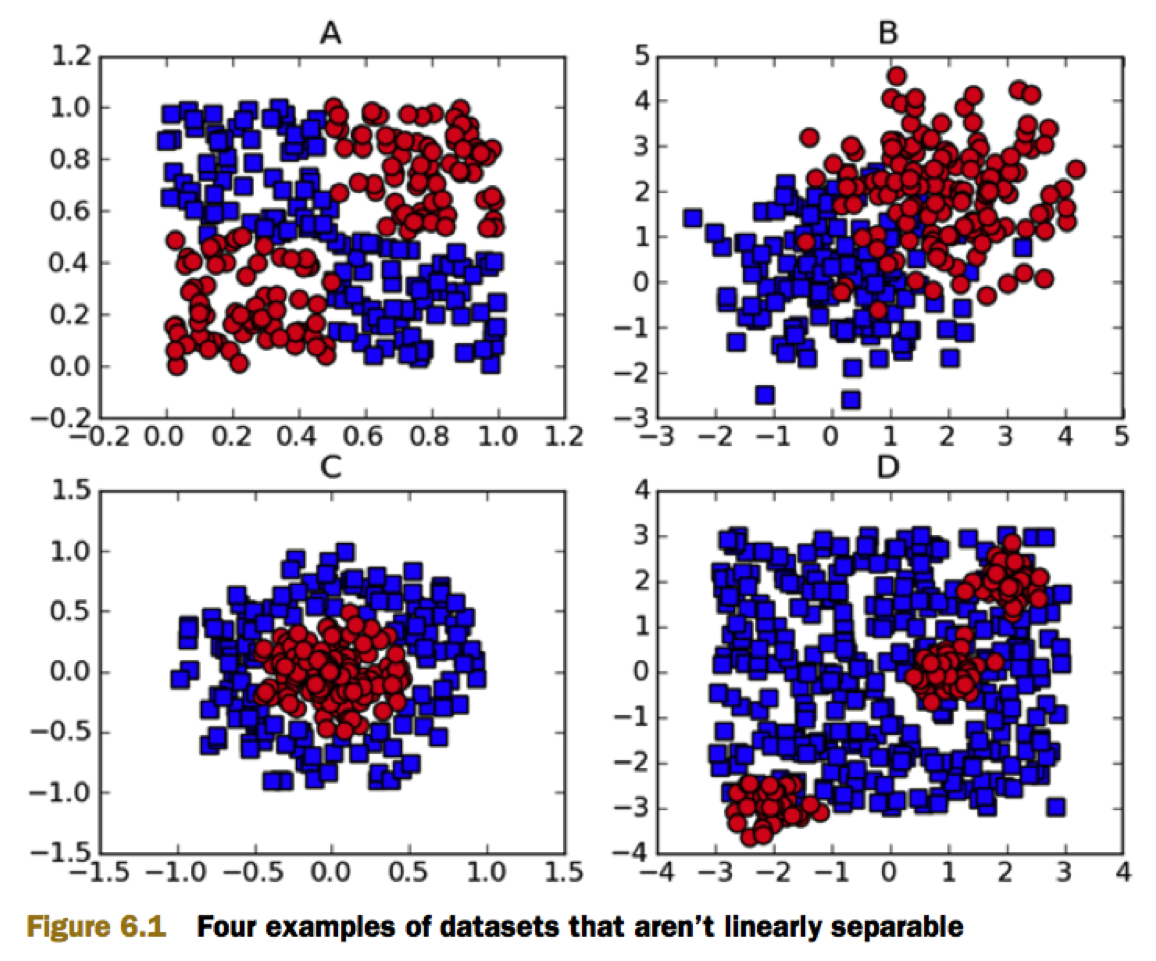
\includegraphics[width=1.0\textwidth]{fig6_1.png}
\caption{\label{fig:svm3}Figure 6.1}
\end{figure}

Support-vector machines let you visualize the prototypes that sit $\pm \epsilon$ around the boundary.  For images, When a new face comes in, it's quite efficient with SVM.  For kNN you would have to compute the distances to every single face.  In SVM, you bring in the new face and do an inner product with the support vectors and if you look at sex classifications for faces in Fig. ~\ref{fig:svm4} you see that these two faces are just $\epsilon$ more or less feminine or masculine.  You can see these exemplars.

A linear SVM probably isn't powerful enough to calculate this.  We need a mechanism to bring in more powerful notions of similarity between patterns.

\begin{figure}
\centering
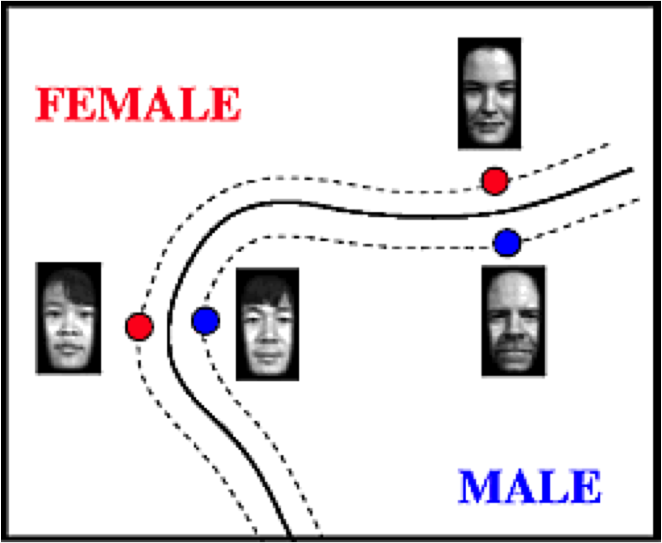
\includegraphics[width=1.0\textwidth]{male_female.png}
\caption{\label{fig:svm4}Male Female}
\end{figure}

\section{Kernels}

What is a kernel? A kernel is a function that satisfies the following conditions:
$$
\sum_{i,j} k(x_i, x_j) c_i c_j \geq 0
$$
for some set of feature vectors $\{x_i\}$ and any vector $c$.

We say the kernel is ``Mercer'' or that it is positive semidefinite. If this were just:
$$
\sum_{i,j} A_{ij} c_i c_j \geq 0 \; or \; equivalently
$$
$$
c^\top A c \geq 0 \; \text{because positive semidefinite} \; A = QQ^\top
$$

If a matrix is positive semidefinite, we can write it as a product of a matrix with its transpose.  Also each entry in a positive semidefinite matrix can be expressed by the pairwise inner products of a set of vectors.

$$
k(x,y) = \phi(x) \dot \phi(y)
$$

The kernel function, $k$, is operating on all data points and pops out numbers for all possible pairs.  If the resulting matrix satisfies the Mercer condition, that means the function $k$ represents an inner product between two vectors. We're generalizing the dot product so if it satisfies this condition, there exists some features vectors that give you the number by computing $k$.  

This is called the ``kernel trick''.  So if you learn a method built around inner products, you look at the algorithm and everywhere it has a dot product, you pull in a kernel instead.  That means you do the algorithm on a higher-dimensional version of the data instead of the data itself.

Whatever $k(x,y)$ is doing, you're lifting the vector into a higher dimensional space.

Let's say $\phi(x)$ represents an empirical feature mapping:
$$
\phi: (x_1, x_2)^\top \rightarrow (x_1, x_2, x_1^2+x_2^2)^\top
$$
$$
x \leftarrow {\rm I\!R}^2, \phi(x) \in {\rm I\!R}^3
$$

Here we went from the native data that is 2-dimensional to mapped 3-dimensional data, supplemented by the sum of squares.

If you imagine a clump with an annulus, the data may not be perfectly linearly separable but by adding a dimension becomes more separable, perhaps with a plane.

\subsection{Examples of Kernels}

\begin{enumerate}
\item
RBF (radial basis function):
$$
k(x,y) = e^{-{\| x-y \|}^2 / \alpha}
$$

\item For histogram data $h_i, g_i$, use $\chi^2$ kernel:
$$
\chi^2 = \frac{1}{2} \sum_{i=1}^{K} \frac{{h_i-g_i}^2}{h_i+g_i}
$$
$$
k(h,g) = e^{-\chi^2(h,g) / \alpha}
$$
\end{enumerate}


There is some $\phi(x)$ that would give you a new vector that if you do the inner product on would give you the same as the kernel.  However, some of these feature mappings would be infinitely long.  

\begin{figure}
\centering
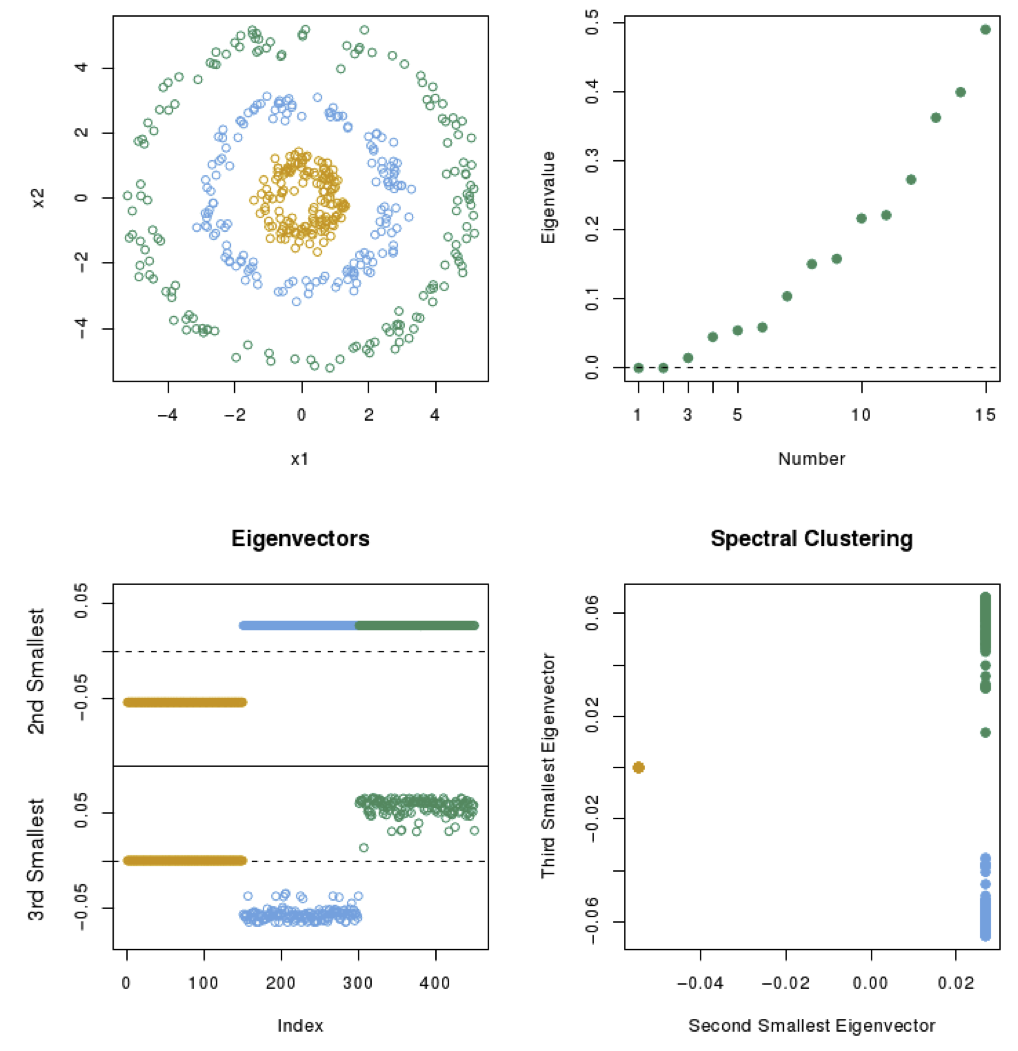
\includegraphics[width=1.0\textwidth]{fig14_29.png}
\caption{\label{fig:kernel}Fig. 14.29}
\end{figure}

The main place you see these things is with SVMs with kernels, kPCA, and spectral clustering.  We can see some of this in Fig. ~\ref{fig:kernel}.  

If you did K-Means with the top left you probably wouldn't get anything useful.  With spectral clustering, you still use K-Means but first evaluate a Gaussian between all pairs of points, creating a kernel matrix using one of the example kernels above.  You get a Gaussian-weighted distance matrix and find its leading eigenvectors and keep the first k.  If you plot the eigenvectors and keep the first k, you do K-Means and then get this nice separation between the clusters.  The first eigenvector separates from the second and the second separates the third.  You still use k-means after producing the kernel matrix and its eigenvectors.  You do clustering on the leading eigenvectors.

\end{document}
